%%
% TUM Corporate Design LaTeX Templates
% Based on the templates from https://www.tum.de/cd
%
% Feel free to join development on
% https://gitlab.lrz.de/tum-templates/templates
% and/or to create an issue in case of trouble.
%
% tum-presentation class for scientific talks, thesis presentations, ...
%
%%

%\documentclass[4to3]{tum-presentation}
%\documentclass[navsym]{tum-presentation}
%\documentclass[nothreeliner]{tum-presentation}
%\documentclass[handout,4on1]{tum-presentation}
%\documentclass[handout,2on1]{tum-presentation}
%\documentclass[handout]{tum-presentation}

\documentclass{tum-presentation}

\usepackage{import}
\usepackage{xifthen}
\usepackage{pdfpages}
\usepackage{transparent}
\usepackage{hyperref}
\usepackage{tcolorbox}
\usepackage{algorithmic}
\usepackage[ruled, lined, linesnumbered, commentsnumbered, longend]{algorithm2e}
% load biblatex
\usepackage[backend=bibtex, sorting=none]{biblatex}
\usepackage{pgfpages}
% set notes

\usepackage{graphics}
\usepackage{xcolor}
\usepackage{pgffor}
\usepackage{tikz}
\usepackage{pgfplots}
\usepackage{amsmath}
\usepackage{pifont}
\usepackage[style=base]{caption}
\usepackage{subfigure}
\usepackage[clock]{ifsym}
\usepackage{fontawesome}
\usepackage{changepage}
\usepackage{booktabs}
\usepackage{tabularx}
\usepackage{longtable}
\usepackage{tabu}
\usepackage{ltxtable}

\addbibresource{literature.bib}

\hypersetup{
	colorlinks=true,
	linkcolor=blue,
	filecolor=magenta,      
	urlcolor=blue,
}

\def\R{{\mathbb R}} 
\def\N{{\mathbb N}} 
\def\E{{\rm E}} 
\def\P{{\rm P}} 
\def\sumi{\sum_{i=1}^n} 
\def\sumj{\sum_{j=1}^n} 

\def\diag{\text{\rm diag}}
\def\tr{\text{\rm tr}}

\def\be{\begin{equation}}
\def\ee{\end{equation}}

\def\bp{\noindent {\it Proof.}\ }
\def\ep{\hfill $\Box$} 
\def\cproof{gray}

\newtheorem{cor}{Corollary}
\newtheorem{prop}{Proposition}
\newtheorem{rem}{Remark}


\def\sign{{\rm sign}}

\def\sp{{\sigma_{\rm p}}}
\def\ia{\Delta I}
\def\ha{\Delta H}
\def\ip{\Delta_{\rm p}I}
\def\hp{\Delta_{\rm p} H}
\def\simp{s_{\rm p}}
\def\qp{q_{\rm p}}

\newcommand{\incfig}[1]{%
	\def\svgwidth{\columnwidth}
	\import{./figures/}{#1.pdf_tex}
}

\DeclareMathOperator*{\argmin}{arg\,min}
\beamertemplatenavigationsymbolsempty
\setbeamercolor{title}{fg=violet}
\setbeamerfont{note page}{size=\large}
\addtobeamertemplate{note page}{\setbeamerfont{itemize/enumerate subbody}{size=\large}}{}
\pdfinclusioncopyfonts=1
\setbeameroption{show notes on second screen}

\title[Shortened Title]{A Novel Information Theoretic Metric for Labeled Trees}
\subtitle{Master Thesis Presentation}

\author[Denys Lazarenko]{\textbf{Denys Lazarenko \inst{1}} \\ Thesis supervisor: Prof. Dr. Tobias Lasser \inst{2} \\ Principal Advisor: Prof. Thomas Bonald \inst{3}}

\institute[]{\inst{1} Department of Mathematics, Technical University of Munich (TUM) \\
\inst{2} Informatics, Technical University of Munich (TUM) \\
\inst{3} Computer Science, Telecom Paris, Institut Polytechnique de Paris} 

\date{21th of April 2021}

\begin{document}

\begin{frame}[noframenumbering]
	\titlepage
	
	\note[item]{
		Good morning to everyone, my name is Denys Lazarenko and I am a student of Mathematics in Data Science Master Degree Program. Today I would like to present you my research, titled as \textbf{A novel Information Theoretic Metric for Labeled Trees}. It was conducted in cooperation with Data Intelligence and Graphs[DIG] team, a group of researchers at Télécom Paris, under the supervision of Professor Thomas Bonald. This work is based on two papers which are going to be published soon(for now they are in arxiv).
	}
\end{frame}

\begin{frame}
  \frametitle{Outline}
  
  \begin{enumerate}
	\item Problem Statement
	\item Related Work
	\item Methodology
	\item Experiments
	\item Results
	\item Conclusions and Future Work
	\note[item]{
		The outline is the following: we will talk about motivation and application of the current work, have a brief overview of existing metrics. Then I present a theoretic background of a novel metric and outcomes from experiments. At the end we are going to analyse the results and to talk about future work and possible improvements.	
	}
\end{enumerate}

\end{frame}

\begin{frame}
	\setcounter{framenumber}{2}
	\frametitle{Introduction}
	\begin{itemize}
		\item \textbf{\textcolor{TUMBlau}{Motivation:}} 
		\begin{itemize}
			\item Compare quantitatively similarity between two trees composed of the same set of leaves.
			\item Existing metrics suffer from different limitations \cite{RF2013}, \cite{Penny1982}. 
		\end{itemize}
	\end{itemize}
	
	\note[item]{
			Trees are one of the most popular data structures in Computer Science because it is easy to implement and understand them. We know well how to analyse, traverse and use them as a base element of more complicated algorithms. Machine Learning is not an exception, where trees serve different purposes: Decision tree, Random Forest or Tree LSTMs. Additionally, it is frequently the case that we need to quantitatively compare similarity between two or more trees that have the same set of leaves but different topologies. 
			To solve this task, numerous metrics were proposed, however, all these metrics either have high complexity or perform well only in a specific domain.  
		}
\end{frame}

\begin{frame}
	\setcounter{framenumber}{2}
	\frametitle{Introduction}
	\begin{itemize}
		\item \textbf{\textcolor{TUMBlau}{Motivation:}} 
		\begin{itemize}
			\item Compare quantitatively similarity between two trees composed of the same set of leaves.
			\item Existing metrics suffer from different limitations \cite{RF2013}, \cite{Penny1982}. 
		\end{itemize}
		
		\item \textbf{\textcolor{TUMBlau}{Application:}} 
		\begin{itemize}
			\item Hierarchical Clustering.
			\item Biology. 
			\item Finance \cite{Papenbrock2011_1000025469}, \cite{Gallegati2008}.
			\item Natural Language Processing \cite{wordnet}.
		\end{itemize}
	\end{itemize}
		
		\note[item]{
				Indeed, the application area is vast. One of the most popular task of unsupervised learning is clustering. The subfamily of clustering algorithms, called hierarchical clustering, is often used in various tasks due to their explainability and adaptivity. 
				
				There is a considerable demand for a good metric that would be able to evaluate performance of hierarchical clustering algorithms and adjust their hyperparameters. 
				
				To tackle this issue, some new metrics were recently introduced: Dasgupta cost and Tree Sampling Divergence distance.
				
				Besides, other areas of application are Biology, Finance and Natural Language Processing. 
		}
\end{frame}

\begin{frame}
	\setcounter{framenumber}{2}
	\frametitle{Introduction}
	\begin{itemize}
		\item \textbf{\textcolor{TUMBlau}{Motivation:}} 
		\begin{itemize}
			\item Compare quantitatively similarity between two trees composed of the same set of leaves.
			\item Existing metrics suffer from different limitations \cite{RF2013}, \cite{Penny1982}. 
		\end{itemize}
		
		\item \textbf{\textcolor{TUMBlau}{Application:}} 
		\begin{itemize}
			\item Hierarchical Clustering.
			\item Biology. 
			\item Finance \cite{Papenbrock2011_1000025469}, \cite{Gallegati2008}.
			\item Natural Language Processing \cite{wordnet}.
		\end{itemize}
		
		\item \textbf{\textcolor{TUMBlau}{Objective:}} 
		\begin{itemize}
			\item The \underline{key question} is to find a metric assessing the similarity between two trees that have the same set of leaves but different topologies. 
			\item Analyse a \underline{novel} Information Theoretic Metric for Labeled Trees named \textbf{Tree Mutual Information (TMI)}.
		\end{itemize}
	\end{itemize}
		
		\note[item]{
			\textbf{\textcolor{TUMBlau}{Our Objective:}} is to find a metric assessing the quality of trees. We therefore propose a novel Information Theoretic Metric for Trees named Tree Mutual Information (TMI).
		}
\end{frame}


\begin{frame}
	\frametitle{Related work}
	
	\textbf{\textcolor{TUMBlauDunkel}{Graph based metrics}}
	\begin{itemize}
		\item \textbf{\textcolor{TUMBlau}{Dasgupta Cost}} \cite{dasgupta2016cost}
		\begin{itemize}
			\item Relies on the structure of a graph.
			\item It is not continuous function.
			\item The tie-breaking problem.
			\item Finding the tree that minimizes the cost function is NP-hard.
		\end{itemize}
	
	\vspace{0.3cm}
	
	\underline{Since we would like to test not only graph based datasets, we are not going to use this metric for the evaluation.}
	\end{itemize}
	
	\pause  
	
	\vspace{0.3cm}
	
	\textbf{\textcolor{TUMBlauDunkel}{Tree based metrics}}
	\begin{itemize}
	\item \textbf{\textcolor{TUMBlau}{Robinson-Faulds}} \cite{ROBINSON} and modifications \cite{Kuhner1994}, \cite{Critchlow1996}. 
		\begin{itemize}
			\item It is not continuous function.
		\end{itemize}
	\item \textbf{\textcolor{TUMBlau}{Tree edited distance.}} \cite{Zhang1989} and modifications \cite{Tai1979}, \cite{Pawlik2011}, \cite{Pawlik2017}. 
		\begin{itemize}
			\item High time complexity: $O(\mid T_1 \mid \mid T_2 \mid  \min(depth(T_1),leaves(T_1))  \min(depth(T_2),leaves(T_2)))$
		\end{itemize}
	
	\vspace{0.3cm}
	
	\underline{	We are going to use RF and TED as a state of the art metrics reference. }
	\end{itemize}
	
	\note[item]{
		Lets have a look on state of the art metrics, some of them are strictly applicable to graphs, while others are rather for a general usage. However, all these metrics have some limitations, lets analyse some of them:
		
		\textbf{Dasgupta cost:}
		Relies on the structure of a graph. It is not a continuous function, since slight changes modify the score significantly.
		
		\underline{Since we would like to test not only graph based datasets, we are not going to use this metric for the evaluation.}
	}

	\note[item]{	
		The following metrics are tree-based \textbf{ CLICK!!!} : 
		
		Robinson–Foulds is a symmetric distance between two trees, which measures the number of branch-splits present in one tree, but not in another, and scores 1 for each division that is not matched.
		
		RF has its well-known shortcomings: by moving a single node in a tree can result in a considerable jump of RF score, but in reality, these trees are almost identical
		
		Another metric to be considered is \textbf{ordered tree edit distance}, which basically optimizes number of operations which are necessary to transform one tree into another. 
		
		There are 3 allowed operations: rename, delete or insert a node
		
		TED metric has a high time and space complexities. The algorithm's efficiency highly depends on the tree shape.
		
		We are going to use RF and TED as a state of the art metrics reference. 
	
	}
\end{frame}


\begin{frame} 
	\frametitle{Methodology}
	\framesubtitle{Clustering}
	\begin{center}
		\includegraphics[width = 10cm]{../figures/cloud_no_annotations.pdf}\hspace{.5cm}\vline\hspace{.5cm}
		\includegraphics[width = 10cm]{../figures/cloud_no_annotations.pdf}
	\end{center}
	\begin{tcolorbox}
	\begin{center}
		What is the {\bf best clustering}?
	\end{center}
	\end{tcolorbox}
	\note[item]{
	In our new method we are trying to tackle these limitations. Let's get some feeling of methodology which lays underneath of it. Let's start from a very simple example: assume that we have a set of data points and we would like to partition it. Obviously, this figure represent a trivial example, where we have only one cluster with all points in it and it does not contain any information. The natural question which arises "What is the {\bf best clustering}?" 
	}
\end{frame}

\begin{frame}	
	\frametitle{Methodology}
	\framesubtitle{Mutual information}
	\begin{center}
		\includegraphics[width = 10cm]{../figures/cloud_cluster_1.pdf}\hspace{.5cm}\vline\hspace{.5cm}
		\includegraphics[width = 10cm]{../figures/cloud_cluster_2.pdf}
	\end{center}
	
	\pause 
	
	$$
	I(X,Y) = H(X) + H(Y) - H(X, Y) = H(Y) - H(Y|X)
	$$
	$$ 
	I(A, B) = 0.93 
	$$   
	\note[item]{	
		To better explain, assume that we partitioned data based on some criteria and we received 3 clusters from both sides which are marked yellow, green and  purple respectively. The only difference between them is one data point which marked red. In left figure it belongs to purple cluster while in the right one to the green one.
	}
	\note[item]{
		Let's calculate a Mutual Information between these two clusterings. \textbf{[CLICK]}
		%This is "the amount of uncertainty remaining about Y after X is known".
		%and thus the right side of the second equation can be read as "the amount of uncertainty in Y, minus the amount of uncertainty in Y which remains after X is known".
		If two random variables $A$ and $B$ are strongly dependant then there is a high degree of Mutual Information.
	}
	\note[item]{
		In this case we have a value of 0.93, but since we are using a not normalised version of metric it can be greater than one. 
	}
\end{frame}


\begin{frame}	
	\frametitle{Methodology}
	\framesubtitle{Mutual information}
	\begin{center}
		\includegraphics[width = 10cm]{../figures/cloud_cluster_1.pdf}\hspace{.5cm}\vline\hspace{.5cm}
		\includegraphics[width = 10cm]{../figures/cloud_trivial.pdf}
		
		\pause
		
		$$ 
		I(A, C) = 1.11 
		$$   
	\end{center}
	\note[item]{
		More in details: consider the following example: from left side we have the same partition as before, but from right side we have an edge case, when each data point represents a separate cluster. If we measure the mutual information between these two partitions \textbf{[CLICK]} then the value will be greater, meaning that we obtain more information, which is obviously does not represent the reality.
	}
	\note[item]{
		This metric is not adjusted for chance and will tend to increase as the number of clusters increases, regardless of the actual amount of information between the two distributions. That is why adjustment for chance is
		necessary.
	}
\end{frame}

\begin{frame} 
	\frametitle{Methodology}
	\framesubtitle{Adjusted mutual information}
	\begin{center}
		\includegraphics[width = 10cm]{../figures/cloud_cluster_1.pdf}\hspace{.5cm}\vline\hspace{.5cm}
		\includegraphics[width = 10cm]{../figures/cloud_cluster_2.pdf}
		$$
		\ia(X,Y) = I(X,Y) - \E(I(X, Y_\sigma)),
		$$
		
		where  $Y_\sigma$ is the random variable $Y \circ \sigma$, for any permutation $\sigma$ of $\{1,\ldots, n\}$, and the expectation is taken over all permutations $\sigma$, chosen uniformly at random. 

	\end{center}
		\note[item]{
			\textbf{SLOW}
			The adjusted mutual information between $X$ and $Y$ is defined by following equation:
			Adjusted version equals to the Mutual Information subtracting the Expected value between $X$ and $Y$ sigma
			where  $Y_\sigma$ is the random variable $Y$ permuted with $\sigma$ (sigma), which is any permutation  of $n$ labels, chosen uniformly at random. 
	}
\end{frame}


\begin{frame} 
	\frametitle{Methodology}
	\framesubtitle{Adjusted mutual information}
	\begin{center}
		\includegraphics[width = 10cm]{../figures/cloud_cluster_1.pdf}\hspace{.5cm}\vline\hspace{.5cm}
		\includegraphics[width = 10cm]{../figures/cloud_cluster_2.pdf}
		$$
		\ia(X,Y) = I(X,Y) - \E(I(X, Y_\sigma)),
		$$
		
		$$
		\ia(A, B) = 0.76
		$$
	\end{center}
	\note[item]{
		Following to this, we conduct the same experiment, but adjusting the metric against chance. We see that we already receive score which is lower than Mutual Information due to subtraction of Expected value.  
	}
\end{frame}


\begin{frame} 
	\frametitle{Methodology}
	\framesubtitle{Adjusted mutual information}
	\begin{center}
		\includegraphics[width = 10cm]{../figures/cloud_cluster_1.pdf}\hspace{.5cm}\vline\hspace{.5cm}
		\includegraphics[width = 10cm]{../figures/cloud_trivial.pdf}
		$$
		\ia(A, C) = 0
		$$
	\end{center}
		\note[item]{
		And with the trivial clustering the score is 0, meaning that it is completely random and it does not contain any information. 
	}
\end{frame}

\begin{frame}
	\frametitle{Methodology}
	\framesubtitle{Mutual information}
	Let $A = \{A_1,\ldots,A_k\}$ and $B = \{B_1,\ldots,B_l\}$  be two partitions of some finite set $\{1,\ldots,n\}$ into $k$ and $l$ clusters, respectively.  $n_{ij} = |A_i \cap B_j|$ is known as the {\it contingency matrix}. 
	
	\vspace{0.5cm}
	
	\begin{equation}
	MI(A, B) = -\sum_{i=1}^k\sum_{j=1}^l \frac {n_{ij}}n \log \frac {n_{ij}}n
	\end{equation}
	
	\vspace{1cm}
	
	\begin{tcolorbox}
		\begin{center}
			This metric is not adjusted for chance and will tend to increase as the number of clusters increases, regardless of the actual amount of information between the two distributions. That is why adjustment for chance is necessary.
		\end{center}
	\end{tcolorbox}
	
	\note[item]{
		More in depth: here we can see a straightforward formula how to calculate MI between two random variables. $A$ and $B$ are two partitions of some finite set into $k$ and $l$ clusters and $n_{ij} = |A_i \cap B_j|$ is the number of samples both in cluster $A_i$ and  cluster $B_j$, also known as {\it contingency matrix}.} 
\end{frame}


\begin{frame}
	\frametitle{Methodology}
	\framesubtitle{Adjusted Mutual Information}
	
	Note that $a_i$ and $b_j$ are  the respective sums of row $i$  and column $j$ of the contingency matrix.

	\begin{align}\label{eq:ami}
	\begin{split}
	&E[MI](A,B) = \sum_{i=1}^k\sum_{j=1}^l \sum_{c = (a_i+b_j - n)^+}^{\min(a_i, b_j)} \\
	&\frac{a_i!b_j!(n-a_i)!(n-b_j)!}
	{n!c!(a_i-c)!(b_j-c)!(n-a_i-b_j+c)!}\frac {c}n \log \frac {c}n.
	\end{split}
	\end{align}
	
	Finally: 
	\begin{equation}
	s(A,B) = MI(A,B) - E[MI](A,B)
	\end{equation}
	
	\vspace{1cm}
	
	\textbf{Complexity}: \textbf{$O(\max(k,l)n)$ }. In particular, it is dominated by the second term and is linear in the number of samples $n$ \cite{romano2014standardized}.
	
	\note[item]{In this slide you can see the formula of expected value of mutual information, which punishes randomness by subtracting expected value.}
	\note[item]{It is also frequent to normalize adjusted mutual information to get a score between 0 and 1. In this work, we only focus on the adjustment step.}
	\note[item]{its complexity is about $O(\max(k,l)n)$, which is quite slow for the large graphs.}
\end{frame}


\begin{frame} 
	\frametitle{Methodology}
	\framesubtitle{Contribution 1: Pairwise adjustment \cite{Lazarenko2021pairwise}}
	We consider permutations $\sigma$ for which there exists $i,j \in \{1,\ldots,n\}$ 
	such that $\sigma(i) = j$ and $\sigma(j) = i$. We think about the set of such permutations $\sigma$ where the samples $i,j$ are drawn uniformly at random in the set $\{1,\ldots,n\}$. We denote by $\sp$ such a random permutation.
	
	\vspace{0.5cm}
			
	We  define the {\it pairwise adjusted mutual information} as:
	$$
	\ip(X,Y) = I(X,Y) - \E(I(X, Y_\sp)).
	$$
	
	\vspace{0.5cm}
	
	We  also define the {\it pairwise adjusted entropy} as:
	$$
	\hp(X) = \ip(X,X) =  H(X) - \E(I(X, X_\sp)).
	$$
	We have $\hp(X) \ge 0$, with equality if and only if  $X$ is constant or equal to some permutation of $\{1,\ldots,n\}$.
	
	\note[item]{
		Having said that, we come up with an improved version of Adjusted Mutual Information. The main assumption: we consider permutations $\sigma$ (sigma) for which there exists $i,j$ from one to $n$ such that $\sigma(i) = j$ and $\sigma(j) = i$. The samples $i,j$ are drawn uniformly at random in the set one to $n$.
	}
	\note[item]{
		We  define the {\it pairwise adjusted mutual information} and {\it pairwise adjusted entropy}. More detailed information can be find in our original paper.
	}
\end{frame}


\begin{frame} 
	\frametitle{Methodology}
	\framesubtitle{Pairwise adjusted mutual information (PAMI)}
	
	A measure of similarity $\simp(A,B)$ between clusterings $A$ and $B$, based on  the pairwise adjusted mutual information $\ip(X,Y)$ between the corresponding random variables $X$ and $Y$. 
	
	\begin{theorem}\label{theo:pairsim}
		We have:
		\begin{align}\label{eq:pami}
		\begin{split}
		\simp(A,B) &=2 \sum_{i=1}^k \sum_{j=1}^l \frac{n_{ij}(n -a_i -b_j + n_{ij})}{n^2}\\
		&\times  \left(\frac{n_{ij}} n \log\frac{n_{ij}}n - \frac{n_{ij} - 1} n \log\frac{n_{ij} - 1}n\right)\\
		& + 2\sum_{i=1}^k \sum_{j=1}^l \frac{(a_i - n_{ij})(b_j - n_{ij})}{n^2}\\
		&\times\left(\frac{n_{ij}} n \log\frac{n_{ij}}n - \frac{n_{ij} + 1} n \log\frac{n_{ij} + 1}n \right).
		\end{split}
		\end{align}
	\end{theorem}
	\note[item]{
		We have an closed form expression for pairwise similarity. 
		
		The time complexity of this formula is  in $O(kl)$. It is independent of the number of samples $n$ in contrast to the standard Adjusted Mutual information, where we summed over one additional index.
		
		As we can see, this metric is much faster then the standard Adjusted Mutual Information.
	}
\end{frame}

\begin{frame} 
	\frametitle{Methodology}
	\framesubtitle{Pairwise adjusted mutual information (PAMI)}
	For real data, we consider the 79 datasets of the benchmark suite \cite{clustering_benchmarks}
	\footnote{See \url{https://github.com/gagolews/clustering_benchmarks_v1}}. We apply to each dataset 10 clustering algorithms.

	\begin{figure}[h]
		\centering
		\includegraphics[width=0.4\textwidth,keepaspectratio=true]{../figures/spearman.pdf}	
		\caption{Spearman correlation.}
	\end{figure}
	
	\note[item]{
		 Next we demonstrate experiments which proves that the novel metric is actually behaves the same way as a standard one. 
		 
		For real data, we consider the 79 datasets. We apply to each dataset 10 common clustering algorithms from sckit-learn and measure similarity. We then compute  the Spearman correlation of the corresponding similarities} 
	\note[item]{
		We observe that the correlation is very high, suggesting again that both notions of adjusted mutual  information tend to provide the same results. For 65 datasets among 79, the Spearman correlation is higher than 95\%.
	}
	
\end{frame}

\begin{frame} 
	\frametitle{Methodology}
	\framesubtitle{Pairwise adjusted mutual information (PAMI)}
	
	The time complexity of this formula is  in $O(kl)$, like mutual information. It is independent of the number of samples $n$, given the contingency matrix.
	
	\begin{figure}[h]
		\centering
		\includegraphics[width=0.4\textwidth,keepaspectratio=true]{../figures/computation_synthetic.pdf}
		\caption{Computation time with respect to    $n$ (mean $\pm$ standard deviation).\label{fig:time}}
	\end{figure}
	
	\note[item]{
	Related to this, we compute run time of metric when the number of samples $n$ grows from $10^2$ (ten power of 2)  to $10^7$ (ten power of 7). The  performance gain brought by pairwise adjustement is significant. In particular, the computation time becomes independent of the number of samples.}
\end{frame}

%\begin{frame} 
%	\frametitle{Methodology}
%	\framesubtitle{Pairwise adjusted mutual information (PAMI)}
%	\begin{figure}[H]
%		\begin{center}
%			\includegraphics[width=0.5\textwidth]{../figures/4-kmeans.pdf}
%			\caption{Evaluation results on the Gaussian mixture model with $M=10$ clusters and $n=50$ elements in each of it. Shows similarity score s(A, B) of different metrics obtained by K-means with different values of K and the ground-truth partitioning.}
%		\end{center}
%	\end{figure}
%	\note[item]{
%		Now let's consider a bit more complex example. This experiment is intended to demonstrate the behaviour of the Adjusted, Pairwise Adjusted, Expected Mutual Information and Entropy in clustering scenario, depending on the parameter $k$ in K-means clustering algorithm. 
%		
%		For this experiment, we generate $M=10$ isotropic Gaussian blobs of equal size $n=50$. Then we apply the K-Means algorithm varying parameter $k$. We measure similarity between predicted and ground-truth clusterings.
%		
%		Results indicates why adjustment against chance plays a crucial role for a correct measurement of information between assignments. It is worth to mention, both mutual information and its adjusted versions correctly identify an optimal number of clusters equals to 10. MI shows score similar to maximum everywhere, despite the growth of parameter $k$. In contrast, AMI and PAMI react correctly to the increase of noise and capture actual "information" between assignments. 
%	}
%\end{frame}

\begin{frame} 
	\frametitle{Methodology}
	\framesubtitle{Hierarchical clustering}
	\begin{center}
		\includegraphics[width = 10cm]{../figures/karate-paris.pdf}
		%\hspace{.5cm}\vline\hspace{.5cm} \includegraphics[width = 4.5cm]{images/karate-ward.pdf}
	\end{center}
	
	\note[item]{
		In this Figure we can see a typical output of hierarchical clustering algorithm - dendrogram, which is a compact representation of the hierarchical structure. The dendrogram $D$ contains the pair of nodes merged through the run of the algorithm. Additionally, each branch is plotted at height $d$, thus all distances must be non-decreasing.
	}

\end{frame}
	
\begin{frame} 
	\frametitle{Methodology}
	\framesubtitle{Comparing trees}
	\begin{center}
		\includegraphics[width = 10cm]{../figures/karate-paris.pdf}\hspace{.5cm}\vline\hspace{.5cm}
		\includegraphics[width = 10cm]{../figures/karate-ward.pdf}
	\end{center}
	\note[item]{
		Frequently, we have two dendrograms as input and would like to understand how similar are they to each other.
	}
\end{frame}


\begin{frame}
	\frametitle{Methodology}
	\framesubtitle{Example}
	\begin{center}
		\includegraphics[width = 10cm]{../figures/caterpilar_tree_level_0-1.png}\hspace{.5cm}\vline\hspace{.5cm}
		\includegraphics[width = 10cm]{../figures/binary_tree_level_0-1.png}
	\end{center}
	
	\note[item]{
		To better explain the second contribution to the current work, I propose to have a look on a simple example. 
		
		We compare a caterpillar tree (left figure) with a fully binary tree (right figure). 
		The leaves here represent partitioning. We start from the trivial clustering where all leaf nodes belong to the same cluster 0.
		
		Intuitively, the best clustering is achieved with 5 clusters in both trees.
		
		%		by expanding all nodes in the left subtree of \textbf{balanced tree} and keeping the right subtree as one complete cluster. It results in 5 clusters: 4 clusters with 1 element and one cluster of 4. Simultaneously, in the \textbf{caterpillar tree} by sequentially making splits till the 5th level, we obtain an identical distribution of nodes. 
		
		Let's see whether our algorithm behaves the same way, as it is expected? 
	}
\end{frame} 

\begin{frame}
	\frametitle{Methodology}
	\framesubtitle{Example}
	\begin{center}
		\includegraphics[width = 10cm]{../figures/caterpilar_tree_level_1-1.png}\hspace{.5cm}\vline\hspace{.5cm}
		\includegraphics[width = 10cm]{../figures/binary_tree_level_1-1.png}
	\end{center}
	\begin{center}
			$AMI(C_1^{1}, C_2^{1}) = 0.26$
			
			$PAMI(C_1^{1}, C_2^{1}) = 0.046$
	\end{center}
	\note[item]{
	As a first step our algorithm make the only possible cut in both trees which results into score growth.
	AMI has score equal to 0.26 and PAMI is around zero point zero five. It is necessary to remember that both metrics are not normalized!
}
\end{frame} 

\begin{frame}
	\frametitle{Methodology}
	\framesubtitle{Example}
	\begin{center}
		\includegraphics[width = 10cm]{../figures/caterpilar_tree_level_2-1.png}\hspace{.5cm}\vline\hspace{.5cm}
		\includegraphics[width = 10cm]{../figures/binary_tree_level_2-1.png}
	\end{center}
	\begin{center}
		$AMI(C_1^{2}, C_2^{2}) = 0.35$
		
		$PAMI(C_1^{2}, C_2^{2}) = 0.052$
	\end{center}
	\note[item]{
		Following this, the next best cut for tree pairs is obtained by going into left subtree of binary tree and making an additional cut in caterpillar tree. It results into grows of total score for AMI and PAMI.
	}

\end{frame} 

\begin{frame}
	\frametitle{Methodology}
	\framesubtitle{Example}
	\begin{center}
		\includegraphics[width = 10cm]{../figures/caterpilar_tree_level_3-1.png}\hspace{.5cm}\vline\hspace{.5cm}
		\includegraphics[width = 10cm]{../figures/binary_tree_level_3-1.png}
	\end{center}
	\begin{center}
		$AMI(C_1^{3}, C_2^{3}) = 0.39$
		
		$PAMI(C_1^{3}, C_2^{3}) = 0.061$
	\end{center}
	
	\note[item]{
		Continuing the process, we see that further cut in binary tree of the cluster with label "2" into 2 subclusters and an additional cut in caterpillar tree increase the score.
	}

\end{frame} 

\begin{frame}
	\frametitle{Methodology}
	\framesubtitle{Example}
	\begin{center}
		\includegraphics[width = 10cm]{../figures/caterpilar_tree_level_4-1.png}\hspace{.5cm}\vline\hspace{.5cm}
		\includegraphics[width = 10cm]{../figures/binary_tree_level_4-1.png}
	\end{center}
	\begin{center}
		$AMI(C_1^{4}, C_2^{4}) = 0.49$
		
		$PAMI(C_1^{4}, C_2^{4}) = 0.071$
	\end{center}	
	\note[item]{
		Finally, we reached the stage from our assumption - 5 clusters in both trees. It is indeed maximum value for both metrics AMI and PAMI.
	}
\end{frame} 

\begin{frame}
	\frametitle{Methodology}
	\framesubtitle{Example}
	\begin{center}
		\includegraphics[width = 10cm]{../figures/caterpilar_tree_level_4-1.png}\hspace{.5cm}\vline\hspace{.5cm}
		\includegraphics[width = 10cm]{../figures/binary_tree_level_5-1.png}
	\end{center}
	\begin{center}
		$AMI(C_1^{4}, C_2^{5}) = 0.27$
		
		$PAMI(C_1^{4}, C_2^{5}) = 0.042$
	\end{center}
	\note[item]{
		If we continue to do further cuts in any tree, it will lead to the degradation in the score. We can clearly see it in these examples. One additional cut in the binary tree reduces AMI and PAMI scores.
	}
		
\end{frame} 

\begin{frame}
	\frametitle{Methodology}
	\framesubtitle{Example}
	\begin{center}
		\includegraphics[width = 10cm]{../figures/caterpilar_tree_level_5-1.png}\hspace{.5cm}\vline\hspace{.5cm}
		\includegraphics[width = 10cm]{../figures/binary_tree_level_4.png}
	\end{center}
	\begin{center}
		$AMI(C_1^{5}, C_2^{4}) = 0.31$
		
		$PAMI(C_1^{5}, C_2^{4}) = 0.041$
	\end{center}
	\note[item]{
	If we make a cut in the caterpillar tree the value drops as well.
	}	
\end{frame} 

\begin{frame}
	\frametitle{Methodology}
	\framesubtitle{Example}
	\begin{center}
		\includegraphics[width = 10cm]{../figures/caterpilar_tree_level_5-1.png}\hspace{.5cm}\vline\hspace{.5cm}
		\includegraphics[width = 10cm]{../figures/binary_tree_level_5-1.png}
	\end{center}
	\begin{center}
		$AMI(C_1^{5}, C_2^{5}) = 0.13$
		
		$PAMI(C_1^{5}, C_2^{5}) = 0.023$
	\end{center}	
	\note[item]{
	And the last possibility, to make a cut in both trees also results into degradation of similarity score. As a result, the maximum score is obtained with the total number of clusters equal to 5, as was expected in the beginning. 
	}	
\end{frame} 

\begin{frame}
	\frametitle{Methodology}
	\framesubtitle{Contribution 2: Tree Mutual Information (TMI)}
	
	\begin{figure}[!ht]
		\centering
		\begin{minipage}{.45\textwidth}
			\centering
			\begin{algorithm}[H]
				\SetAlgoLined
				\KwIn{initial assignment $C_1$ and $C_2$, trees $T_1$ and $T_2$, set of nodes $V_1=\{root(T_1)\}$ and $V_2=\{root(T_2)\}$, maximum score $S^{max}=-1$}
				\KwOut{Score $S^{max}$}
				\tcp{returns a maximizing pair of nodes and a corresponding clustering}
				$S, T_1, T_2, C_1, C_2 = split(V_1, V_2, C_1, C_2)$\;
				\tcp{stop criteria}
				\If{$S<S^{max}$}{
					return $S^{max}$
				}
				\tcp{updates sets of nodes}
				$V_1 \leftarrow V_1  \backslash T_1$;  $V_1 \leftarrow V_1 \cup cut(T_1)$\;
				$V_2 \leftarrow V_2  \backslash T_2$;  $V_2 \leftarrow V_2 \cup cut(T_2)$\;
				return $TMI(C_1, C_2, V_1, V_2, S)$ 
				\caption{Tree Mutual Information(TMI)}
			\end{algorithm}
		\end{minipage}
		\hfill
		\begin{minipage}{.45\textwidth}
			\centering
%			TODO uncomment
						\begin{algorithm}[H]
							\SetAlgoLined
							\KwIn{$C_1$, $C_2$, $V_1$, $V_2$}
							\KwOut{returns maximum value, a maximizing pair of nodes and a corresponding clustering $S^{max}, V_1^{max}, V_2^{max}, C_1^{max}, C_2^{max}$}
							\For{$node_1 \in V_1$} {
								$C_1 \leftarrow clustering(node_1)$ \;
								\For{$node_2 \in V_2$} 
								{$C_2 \leftarrow clustering(node_2)$ \;
									$S = similarity(C_1, C_2)$ \;
									\If{$S>S^{max}$}{
										$C_1^{max}, C_2^{max}, V_1^{max}, V_2^{max}$ = $C_1, C_2, V_1, V_2$ \;
									}    
								}
								\EndFor
							}
							\EndFor
							return $S^{max},C_1^{max}, C_2^{max}, V_1^{max}, V_2^{max}$ \;
							\caption{split}
						\end{algorithm}
		\end{minipage}
	\end{figure}
	
	
	\note[item]{
		After we understand the logic of a new metric on the simple experiment let's move to the actual algorithm.
		The algorithm takes as input a pair of trees $T_1$ and $T_2$ in Newick format \cite{newick1990} with the same number of leaves $n$ and performs the following steps:
		
		\begin{enumerate}
			\item The TMI algorithm is initialized with 2 sets of nodes which we use to compare on every step: $V_1$ and $V_2$ for each of tree. Additionally, it takes as input maximum score $S^{max}$ and clustering for each leaf set.
			\item Let's look into $split$ algorithm on the right. We consider the clustering $C_1$ induced by the top level of tree $T_1$, and clustering $C_2$ for tree $T_2$ respectively. Compute similarity $S$ between these clusters, where $similarity$ is one of our metrics: AMI or PAMI. If newly computed score $S$ is greater than maximum value $S^{max}$ then we update maximum clusterings with new values.
			\item We repeat recursively the step above, meaning whenever score $S$ increases, we change clustering going down in tree $T$ and making cut.
			\item If on the step $i$ no cut in trees $T_1$ and $T_2$ increases the score $S^{max}$ then we hit the stop criteria and return maximum value $S$.
		\end{enumerate}
	}
\end{frame}


\begin{frame} 
	\frametitle{Methodology}
	\framesubtitle{Optimal number of partitions}
	\begin{block}{Conjecture}
		For a large number of items $n$, the adjusted entropy is maximized for $\sqrt{n}$ clusters of same size
		\label{conjecture}
	\end{block}
	
	\begin{center}
		\begin{figure}
			\subfigure[Intrinsic information of a clustering of $n=100$ items into $k$ clusters, with respect to $k$.]{
				\includegraphics[width=9cm]{../figures/info-100.pdf}
				\label{intrinsic_information}
			}
			\subfigure[Optimal number of clusters with respect to  $n$.]{
				\includegraphics[width=9cm]{../figures/sqrt.pdf}
				\label{optimal_n_clusters}
			}	
		\end{figure}
	\end{center}
	
	\note[item]{
		Following Conjecture suggests that for a large number of items $n$, the adjusted entropy is maximized for $\sqrt{n}$ clusters of same size. 
		
		We justify the best cut property by following experiments. 
		

		
		We take a randomly generated dataset of different size $n$. Then we partition it in $K$ clusters in the range $\{1,\ldots, n\}$. We measure adjusted entropy for each set of labels. In Figure 1, we can clearly see that the peak of shared information to the number of clusters equals 10. To identify an optimal number of clusters, we take the maximum index of all adjusted entropy scores. We can notice that in Figure 2 the optimal number of clusters and a squared root function have almost identical behaviour.
		
		We can extend this Conjecture further to the similarity $s$ between clusterings $A$ and $B$. 
	}
\end{frame}

\begin{frame} 
	\frametitle{Methodology}
	\framesubtitle{Complexity}
	
	Let's consider trees $T1$ and $T2$ with n-leaves. Let $A_i = \{A_{i1},\ldots,A_{ik_i}\}$ and $B_j = \{B_{j1},\ldots,B_{jl_j}\}$ be two partitions on trees' levels $i$, $j$ of some finite set $\{1,\ldots,n\}$ into $k_i$ and $l_j$ clusters, respectively. According to Conjecture the optimal numbers of clusters $k$ and $l$ are not exceeded by $\sqrt{n}$  in practice. We can get an approximation of complexity:
	
	$$
	T(n) = O(n^{2.5})
	$$
	for a Tree Mutual Information with AMI metric(TAMI)  
	
	$$
	T(n) = O(n^{1.5})
	$$
	and for Tree Mutual Information with PAMI metric(TPAMI).   
	
	\note[item]{
		To provide a closed form solution of algorithm complexity, we need to solve a discrete optimization problem which is not trivial. Hence, we are going to derive an approximated bound for the new metrics.  
		
		Let's consider trees $T1$ and $T2$ with n-leaves. Let $A_i$ and $B_j$ be two partitions on trees' levels $i$, $j$ into $k_i$ and $l_j$ clusters, respectively.
	}
	
	\note[item]{
		Complexity of $split$ operation includes two nested loops $V_1$ and $V_2$ which on each step calculate metric AMI or PAMI. According to Conjecture the optimal numbers of clusters $k$ and $l$ are not exceeded by $\sqrt{n}$ in practice. We can get an approximation of complexity on the following parts:
		
		$$
		T(n) = O(n^{2.5})
		$$
		for a Tree Mutual Information with AMI metric 
		
		$$
		T(n) = O(n^{1.5})
		$$
		for PAMI metric.   
	}
\end{frame}


\begin{frame} 
	\frametitle{Experiments}
	\framesubtitle{Settings}
	
	\textbf{\textcolor{TUMBlau}{Metrics requirements}}
	\begin{itemize}
		\item Similarity.
		$$
		 \text{Pearson correlation} = \frac{\sum(x-m_x)(y-m_y)}{\sqrt{\sum(x-m_x)^2 \sum(y-m_y)}}
		$$
		,where $m_x$ os the mean of the vector $x$ and $m_y$ is the mean of vector $y$.
		
		\pause
		
		\item Time complexity.
		
		\pause
		
		\item Optimal partitioning.
	\end{itemize}

	\vspace{0.5cm}
	\pause
	
	\textbf{\textcolor{TUMBlau}{Agglomerative hierarchical clustering algorithms}}
		\begin{itemize}
		\item Ward \cite{Ward1963}.
		\item Louvain \cite{Newman_2004}.
		\item Paris  \cite{Bonald2018}.
	\end{itemize}

	
	\note[item]{
		To justify effectiveness of proposed algorithm, we are moving to experiments. We test metrics in various scenarios and datasets: synthetic datasets give us a possibility to analyse the behaviour of metrics on simple examples. In contrast, real datasets help to understand the scaling and generalisation potential.  
		We introduce the following requirements. }
	
	
	\note[item]{
		1) To capture quantitatively behaviour of metrics in the syntactic experiments, we measure the Pearson correlation between values of corresponding metric and numbers of shuffled pairs. We expect this correlation to be high. \textbf{[CLICK]}
		
		2) Our metric should scale on large datasets. We would like to have a clear understanding on how it grows with the increasing number of samples. Therefore, we will measure time complexity and expect it to be low. \textbf{[CLICK]}
	
		3)  Another critical aspect for the metric is to be explainable, therefore we analyse dependency of the optimal number of clusters to the similarity score. \textbf{[CLICK]} 
		
		We will use following agglomerative clustering algorithms: Ward, Louvain and Paris. They all works with graph and vector data.
	}
\end{frame}


\begin{frame} 
	\frametitle{Experiments}
	\framesubtitle{Syntactic data: Binary Trees}
	\begin{figure}[H]
		    \centering
		\begin{minipage}{.6\textwidth}
			\begin{center}
				\includegraphics[width=0.7\textwidth]{../figures/1-syntatic-trees-binary.pdf}			
				\caption{Binary trees with $n=100$ leaves: dependence of the similarity score to the parameter $k$ - shuffled leaves pairs.}
			\end{center}
		\end{minipage}%
		\begin{minipage}{0.4\textwidth}
			\begin{table}
				\centering
				\caption{Pearson correlation between number of leaf shuffled pairs and values of corresponding metric.}
				\input{../tables/1-syntatic-tree-corr.tex}.
			\end{table}
		\end{minipage}
	\end{figure}
	\note[item]{
		Having said this, the first experiment is conducted in the following settings: a binary tree with 100 leaves is generated, and we introduce parameter $k$ - a number of shuffled leaf pairs. Afterwards, we shuffle leaves and measure similarity between the original tree and permuted one. 
	}
	\note[item]{
		 As we can see, all algorithms capture the trend correctly: with an increasing number of shuffled leaf pairs $k$, the similarity between trees decreases. 
		 
		% It is critical to highlight that experiments are conducted on the same tree structure, only leaves names are shuffled. This influences explicitly TED metrics' behaviour, which in this scenario turns into a string-to-string problem and shows a perfect performance. Later, we will see that it is not the case when tree structure varies.         
		
		To prove quantitatively the statement above, we measure the Pearson correlation. The correlation Table demonstrates that the TED metric perfectly correlates with noise, while TAMI and TPAMI have scores around $-0.96$ which is almost perfect. The worst performance has the RF metric.
	}
	
\end{frame}

\begin{frame} 
	\frametitle{Experiments}
	\framesubtitle{Syntactic data: Binary Trees}
\begin{figure}[H]
	\centering
	\subfigure{
		\centering
		\includegraphics[width=0.47\textwidth]{../figures/1-syntatic-binary-tree-time-vs-n-leaves.pdf}
		\label{fig:binary_tree_shuffled_time_to_n_leaves_}
	}
	\subfigure{
		\centering
		\includegraphics[width=0.46\textwidth]{../figures/1-syntatic-binary-tree-time-vs-n-leaves-zoom.pdf}
		\label{fig:binary_tree_shuffled_time_to_n_leaves_zoom}
	}
	\caption{Time complexity between two randomly generated binary trees depending on the $n$ number of leaves.}
	\label{fig:binary_tree_shuffled_time_to_n_leaves}
\end{figure}
	\note[item]{
		Following to this, we would like to understand how time complexity changes with the leaves' number $n$.  We randomly generate a pair of binary trees with $n$ leaves and measure the time needed for the metrics to be calculated.
		The results are following:
		\begin{itemize}
			\item TED metric has huge time complexity on relatively small trees -> left Figure.  
%			As mentioned in the beginning, its complexity depends on the number of leaves and each tree's depth, which equals $log(n)$ for binary trees, that results in high complexity. 
			\item While TAMI is significantly faster in comparison to TED, it is one order slower than TPAMI -> right Figure.
			\item TPAMI and RF metrics have a similar performance. 
		\end{itemize}
	}

\end{frame}


%\begin{frame} 
%	\frametitle{Experiments}
%	\framesubtitle{Syntactic data: General Trees}
%	\begin{figure}[H]
%	\centering
%	\begin{minipage}{.6\textwidth}
%		\begin{center}
%			\includegraphics[width=0.7\textwidth]{../figures/1-syntatic-trees-general.pdf}			
%			\caption{General trees with $n=100$ leaves: dependence of the similarity score to the parameter $k$ - shuffled leaves pairs.}
%		\end{center}
%	\end{minipage}%
%	\begin{minipage}{0.4\textwidth}
%		\begin{table}
%			\centering
%			\caption{Pearson correlation between two randomly generated binary trees depending on the $n$ number of leaves.}
%			\begin{tabular}{rrrr}
\toprule
    TAMI &     TPAMI &        RF &  TED \\
\midrule
-0.97592 & -0.970041 & -0.814345 & -1.0 \\
\bottomrule
\end{tabular}
.
%		\end{table}
%	\end{minipage}
%	\end{figure}
%	
%	\note[item]{
%		This is a similar experiment, but instead of binary trees, general trees are considered. 
%		Results from Figure and Table gives us the following insights:
%		\begin{itemize}
%			\item TED, TAMI, and TPAMI metrics show high correlation scores, meaning that similarity consistently decreases with a growing number of permutations.
%			\item In contrast to binary experiment, RF metric does not behave coherently: it drops to 0 with a small amount of noise and jumps when a number of permutations increases. Overall, its performance is unstable, indicating that RF fails to capture dependency between original and tree with noise. 
%		\end{itemize}
%	}
%\end{frame}
%
%\begin{frame} 
%	\frametitle{Experiments}
%	\framesubtitle{Syntactic data: General Trees}
%	\begin{figure}[H]
%		\begin{center}
%			\includegraphics[width=0.5\textwidth]{../figures/1-syntatic-general-tree-time-vs-n-leaves.pdf}
%			\caption{Time complexity between two randomly generated general trees depending on the $n$ number of leaves.}
%			\label{fig:general_tree_shuffled_time_to_n_leaves}
%		\end{center}
%	\end{figure}
%	\note[item]{
%		Time complexity results explain us the following:
%		\begin{itemize}
%			\item All metrics have lower time complexities on general trees in contrast to binary trees.
%			\item TAMI has the worst complexity and proves its theoretic estimation of $O(n^{2.5})$ (O n power two point five).
%			\item Due to the lower tree depth of general trees, time complexity for TED is better than in previous experiment and it outperforms TAMI.  
%			\item TPAMI and RF have the lowest numbers in comparison to others.
%		\end{itemize}
%	}
%\end{frame}

\begin{frame} 
	\frametitle{Experiments}
	\framesubtitle{Syntactic data: Stochastic Block Model (SBM)}
	\begin{itemize}
		\item \textbf{\textcolor{TUMBlau}{Input:}} unlabeled graph $G=(V,E)$ (directed, undirected, bipartite) represented as adjacensy matrix $A$.
		\item \textbf{\textcolor{TUMBlau}{Output:}} hierarchy of clusters represented as a dendrogram $D$.
	\end{itemize}
	\begin{figure}[H]
		\begin{center}
			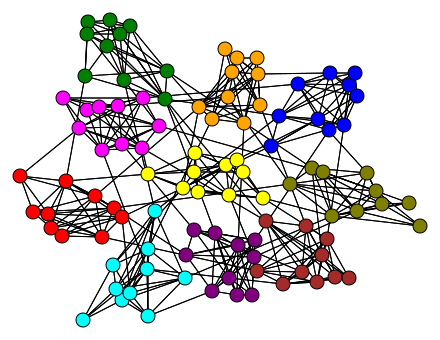
\includegraphics[width=0.37\textwidth]{../figures/2-block-model-sbm-graph.pdf}
			\caption{SBM graph with $n=100$ nodes, $p_{in}=1$, $p_{out}=0.01$ and $K=10$ classes which are uniformly distributed. There are 381 edges with an avarage degree of 7.62.}
			\label{fig:sbm_graph}
		\end{center}
	\end{figure}
	\note[item]{
		The next experiment is based on Stochastic Block Model. SBM is a generative model that produces graphs with communities. It creates graphs with $n$ nodes that are grouped into $k$ sets.
	}
	\note[item]{
		 So, we generate the graph $G_{origin}$ with $n=100$ nodes and $K=10$ clusters. 
%		 It results in the graph, which has 381 edges and an average degree of 7.6.
	}
\end{frame}


\begin{frame} 
	\frametitle{Experiments}
	\framesubtitle{Syntactic data: SBM}
	\begin{figure}[h]
		\centering
		\subfigure[Ground-truth dendrogram.]{
			\centering
			\includegraphics[width=0.46\textwidth,keepaspectratio=true]{../figures/2-block-model-sbm-dendrogram_ground_truth.pdf}
			\label{fig:sbm_dendeogram_original}
		}
		\subfigure[Dendrogram obrained after applying the Ward algorithm.]{
			\centering
			\includegraphics[width=0.46\textwidth,keepaspectratio=true]{../figures/2-block-model-sbm-dendrogram_Ward.pdf}
			\label{fig:sbm_dendeogram_ward_}
		}
%		\caption{Dendrogram \ref{fig:sbm_dendeogram_original} is syntactically generated, while \ref{fig:sbm_dendeogram_ward_}, obtained by applying clustering algorithms to the SBM graph.}
	\end{figure}
	\note[item]{
		 Then we construct a ground truth hierarchy of the given graph represented as a dendrogram $D_{origin}$, which for simplicity has only one level and 10 clusters with 10 nodes in each of them. Other 3 dendrograms are obtained by applying Ward, Louvain and Paris algorithms.
	}
\end{frame}


\begin{frame} 
	\frametitle{Experiments}
	\framesubtitle{Syntactic data: SBM}
	\begin{figure}[h]
		\centering
		\subfigure[Dendrogram obrained after applying the Louvain algorithm.]{
			\centering
			\includegraphics[width=0.46\textwidth,keepaspectratio=true]{../figures/2-block-model-sbm-dendrogram_Louvain.pdf}
			\label{fig:sbm_dendeogram_louvain_}
		}
		\subfigure[Dendrogram obrained after applying the Paris algorithm.]{
			\centering
			\includegraphics[width=0.46\textwidth,keepaspectratio=true]{../figures/2-block-model-sbm-dendrogram_Paris.pdf}
			\label{fig:sbm_dendeogram_paris_}
		}
	\end{figure}
\end{frame}

\begin{frame} 
	\frametitle{Experiments}
	\framesubtitle{Syntactic data: SBM}
	\begin{figure}[H]
		\centering
		\begin{minipage}{.6\textwidth}
			\begin{center}
				\includegraphics[width=0.7\textwidth]{../figures/2-block-model-sbm-Ward.pdf}			
				\caption{Similarity results on the Ward dendrogram.}
			\end{center}
		\end{minipage}%
		\begin{minipage}{0.4\textwidth}
			\begin{table}
				\centering
				\caption{SBM - Pearson correlation between amount of noise and values of corresponding metric.}
				\begin{tabular}{lr}
					\toprule
					{} &      Ward  \\
					\midrule
					TAMI  & -0.948200 \\
					TPAMI & -0.956005 \\
					RF    & -0.857013 \\
					TED   & -0.791978 \\
					\bottomrule
				\end{tabular}
			\end{table}
		\end{minipage}
	\end{figure}
	
	\note[item]{
		 We add noise $p_{shuffled}$ by randomly shuffling edges between nodes in the original graph $G_{origin}$,After applying clustering algorithms: Ward, Louvain and Paris hierarchies of different qualities are obtained. Then we measure similarity.
	}
	\note[item]{
%		In this experiment the structure of the trees changes
%		, therefore we do not see anymore perfect correlation of TED metric. TPAMI has the best performance in terms of Pearson correlation.
		
		TMI with AMI and PAMI behaves very similar in all experiments and outperforms two other metrics. These functions behave smoothly and coherent. 
		
		In contrast, RF and TED behave very differently depending on the algorithm, which resembled in Pearson correlation score: both metrics show an unstable performance from one algorithm to another. For example, with the Ward clustering algorithm, they can capture similarity with a little amount of noise, but when it reaches the point $p_{shuffle}=0.4$ both metrics drop to values around 0 and have some spikes when noise is high. 
	}
\end{frame}

\begin{frame} 
	\frametitle{Experiments}
	\framesubtitle{Syntactic data: SBM}
	\begin{figure}[H]
		\centering
		\begin{minipage}{.6\textwidth}
			\begin{center}
				\includegraphics[width=0.7\textwidth]{../figures/2-block-model-sbm-Louvain.pdf}			
				\caption{Similarity results on the Louvain dendrogram.}
			\end{center}
		\end{minipage}%
		\begin{minipage}{0.4\textwidth}
			\begin{table}
				\centering
				\caption{SBM: Pearson correlation between amount of noise and values of corresponding metric.}
				\begin{tabular}{lr}
					\toprule
					{} &    Louvain  \\
					\midrule
					TAMI  & -0.961134 \\
					TPAMI & -0.962542 \\
					RF    & -0.869449 \\
					TED   & -0.887756 \\
					\bottomrule
				\end{tabular}
			\end{table}
		\end{minipage}
	\end{figure}
	\note[item]{
		Similar behaviour is observed for Lauvain algorithm.
	}
\end{frame}

\begin{frame} 
	\frametitle{Experiments}
	\framesubtitle{Syntactic data: SBM}
	\begin{figure}[H]
		\centering
		\begin{minipage}{.6\textwidth}
			\begin{center}
				\includegraphics[width=0.7\textwidth]{../figures/2-block-model-sbm-Paris.pdf}			
				\caption{Similarity results on the Paris dendrogram.}
			\end{center}
		\end{minipage}%
		\begin{minipage}{0.4\textwidth}
			\begin{table}
				\centering
				\caption{SBM: Pearson correlation between amount of noise and values of corresponding metric.}
				\begin{tabular}{lr}
					\toprule
					{} &    Paris  \\
					\midrule
						TAMI  & -0.959607 \\
						TPAMI & -0.964492 \\
						RF    & -0.771732 \\
						TED   & -0.817506 \\
					\bottomrule
				\end{tabular}
			\end{table}
		\end{minipage}
	\end{figure}
	\note[item]{ 
		By using the Paris clustering algorithm, the final results are very unstable: RF shows almost always 0 similarity everywhere except for few spikes. Tree Edited Distance shows very high similarity even with a high amount of noise. These two metrics behave unstably and fail to capture actual dependence.
	}
\end{frame}

\begin{frame} 
	\frametitle{Experiments}
	\framesubtitle{Syntactic data: SBM}
	\begin{table}[H]
		\centering
		\caption{Evaluation results on the SBM graph measuring optimal number of clusters between hierarchies represented by dendrograms $D_{original}$ and $D_{shuffled}$ depending on amount of noise $p_{shuffled}$. Tree Mutual Information with AMI and PAMI metrics are compared. \label{fig:sbm_results_n_clusters}}
		\subfigure[TAMI.]{
			\centering
			\small\addtolength{\tabcolsep}{-1pt}
			\begin{tabular}{llllllllllll}
\toprule
{} &       0.0 &       0.1 &       0.2 &       0.3 &       0.4 &       0.5 &       0.6 &       0.7 &       0.8 &       0.9 &       1.0 \\
\midrule
Ward    &  [10, 10] &  [10, 10] &  [10, 10] &   [10, 8] &   [10, 9] &  [10, 13] &  [46, 24] &  [37, 16] &  [64, 19] &  [37, 11] &  [46, 24] \\
Louvain &  [10, 10] &  [10, 10] &  [10, 10] &  [10, 11] &  [10, 12] &  [10, 12] &  [19, 14] &  [37, 41] &  [28, 21] &  [37, 25] &  [55, 38] \\
Paris   &  [10, 10] &  [10, 10] &  [10, 10] &  [10, 10] &  [19, 10] &   [10, 9] &  [46, 13] &  [37, 16] &  [64, 21] &  [64, 23] &  [64, 23] \\
\bottomrule
\end{tabular}
 
		}
		\subfigure[TPAMI.]{
			\centering
			\small\addtolength{\tabcolsep}{-1pt}
			\begin{tabular}{llllllllllll}
\toprule
{} &       0.0 &       0.1 &       0.2 &       0.3 &       0.4 &       0.5 &       0.6 &       0.7 &       0.8 &       0.9 &       1.0 \\
\midrule
Ward    &  [10, 10] &  [10, 10] &  [10, 10] &   [10, 8] &   [10, 6] &  [10, 13] &  [28, 26] &   [37, 7] &   [46, 8] &  [37, 11] &  [46, 20] \\
Louvain &  [10, 10] &  [10, 10] &  [10, 10] &   [10, 9] &   [10, 8] &  [10, 12] &  [10, 21] &  [37, 36] &  [37, 30] &  [37, 24] &  [46, 23] \\
Paris   &  [10, 10] &  [10, 10] &  [10, 10] &  [10, 10] &  [19, 10] &   [10, 9] &  [46, 10] &  [37, 11] &  [55, 15] &   [55, 2] &   [55, 9] \\
\bottomrule
\end{tabular}

		}
	\end{table}
	\note[item]{
		More in deep, in the Table (a) and (b) we can see dependency of optimal number of clusters for each tree, corresponding to the algorithm and the amount of noise $p_shuffled$. Now, lets analyse it:
		\begin{itemize}
			\item TAMI and TPAMI identify the optimal number of clusters equal to 10 as in ground truth dedndrogram when the amount of noise is less than 0.3.
			\item However, when noise is bigger than 0.5, fluctuation in the optimal number of clusters is quite significant for both metrics.
%			\item It worth mentioning that TPAMI tends to show smaller numbers and stop earlier without going too deep into a tree structure in contrast to the TAMI metric. 
		\end{itemize} 
	}
\end{frame}

\begin{frame} 
	\frametitle{Experiments}
	\framesubtitle{Real datasets}
		\begin{figure}[H]
		\centering
		\begin{minipage}{.4\textwidth}
			\begin{center}
				\includegraphics[width=7cm]{../figures/openflights_visualization.png}			
				\caption{OpenFlights graph.}
			\end{center}
			\begin{table}
				\caption{Summary of the 2 datasets}
				\label{openflights_trees_information}
				\begin{tabular}{lrrr}
\toprule
Dataset &  nodes &  edges &  average degree \\
\midrule
OpenFlight  &  3097 &     18193 &   11.74 \\
WikiVitals  &  10012 &    792091 &  158.22 \\
\bottomrule
\end{tabular}


			\end{table}

		\end{minipage}%
		\begin{minipage}{0.6\textwidth}
			\begin{table}
				\caption{Openflights: trees information.}
				\label{openflight_trees_information}
				\begin{tabular}{lrrr}
\toprule
{} &  Ward &  Louvain &  Paris \\
\midrule
Number of leaf nodes  &  3097 &     3097 &   3097 \\
Total number of nodes &  6005 &     4274 &   6193 \\
Most distant node     &   237 &     3053 &   1706 \\
Max. distance         &    24 &        7 &     32 \\
\bottomrule
\end{tabular}

			\end{table}
			\begin{table}
				\caption{WikiVitals: trees information.}
				\label{openflight_trees_information}
				\begin{tabular}{lrrrr}
\toprule
{} &  Ground Truth &   Ward &  Louvain &  Paris \\
\midrule
Number of leaf nodes  &         10012 &  10012 &    10012 &  10012 \\
Total number of nodes &         11319 &  20023 &    14231 &  20023 \\
Most distant node     &         10011 &   4924 &     9516 &   7650 \\
Max. distance         &             5 &     23 &       10 &     84 \\
\bottomrule
\end{tabular}

			\end{table}
		\end{minipage}
	\end{figure}
	\note[item]{
		Next, we show the practical interest of TMI in terms of tree comparison. The experiments on real networks are performed on 2 datasets with various sizes and sparsity.
	}
	\note[item]{
		We conduct these experiments only with newly developed metrics. We disregard RF and TED metrics due to bad performance in the clustering scenario and inefficiency for large datasets.  
	}
	\note[item]{
		OpenFlights is a weighted graph in which nodes represent airports and edges the number of flights. \textbf{We do not have a ground truth dendrogram for this graph. }
		
		The Wikivitals dataset is an unweighted graph where nodes represent Vital articles of Wikipedia .\textbf{ We reconstruct the hierarchy from ground truth labels:} and use for evaluation.
	}
	\note[item]{
		We apply all three algorithms to the datasets and obtain trees with the following statistics, which you can observe in Tables on the right. We can see that the structure of these trees is very different.
	}
\end{frame}

\begin{frame} 
	\frametitle{Experiments}
	\framesubtitle{Real datasets: WikiVitals}
	\begin{table}[H]
		\centering
		\caption{WikiVitals: similarity matrix.}
		\subfigure[TAMI.]{
			\centering
			\begin{tabular}{lrrrr}
\toprule
{} &  Ward &  Paris &  Louvain &  Wikivitals \\
\midrule
Ward       &  3.99 &   2.06 &     2.52 &        2.10 \\
Paris      &  2.06 &   3.95 &     2.18 &        1.93 \\
Louvain    &  2.52 &   2.18 &     3.92 &        2.15 \\
Wikivitals &  2.10 &   1.93 &     2.15 &        3.87 \\
\bottomrule
\end{tabular}
 
		}
		\subfigure[TPAMI.]{
			\centering
			\begin{tabular}{lllll}
\toprule
{} &  Ward & Paris & Louvain & WikiVitals \\
\midrule
Ward       &  3.52 &  1.83 &    2.18 &       1.79 \\
Paris      &  1.83 &  3.53 &    1.82 &       1.68 \\
Louvain    &  2.18 &  1.82 &    3.49 &       1.8 \\
WikiVitals &  1.79 &  1.68 &    1.8 &        3.5 \\
\bottomrule
\end{tabular}

		}
	\end{table}
	
	\begin{table}[H]
		\centering
		\caption{WikiVitals: time complexities (s). \label{openflight_time}}
		\subfigure[TAMI.]{
			\centering
			\input{../tables/ami_wikivitals_results_with_louv_depth_20_time.tex} 
		}
		\subfigure[TPAMI.]{
			\begin{tabular}{lllll}
\toprule
{} & Ward & Paris & Louvain & WikiVitals \\
\midrule
Ward       &    4 &   372 &     117 &        181 \\
Paris      &  372 &     3 &    1089 &        402 \\
Louvain    &  117 &  1089 &       1 &        275 \\
WikiVitals &  181 &   402 &     275 &          1 \\
\bottomrule
\end{tabular}

		}
	\end{table}
	\note[item]{
		 In order to spare the time I will only present results of WikiVitals dataset, where we know ground truth dendrogram. We compare all these dendrograms with each other. From the similarity matrix, we observe that both metrics TAMI and TPAMI identify the Louvain tree as the most similar to ground truth, while Ward takes the second spot and the Paris tree has the worst similarity rate. The outcome that the Louvain tree is the most similar to ground truth is not surprising, because they have alike structure: Louvain has only 7 levels of hierarchy and they are subdivided in the "general tree" way, meaning the number of clusters is not limited to be divided by 2. In the ground truth tree has 5 levels with similar properties. Two other algorithms: Ward and Paris tend to produce structure resembling binary tree. 
%		Overall, results for both metrics are pretty similar, the only noticeable difference is that TAMI finds the pair (Ward, Paris) less similar than (Ward, Wikivitals).
	}
	\note[item]{
		The Table with time complexities presents us run time of each metric on certain dendrogram. TPAMI works much faster than TAMI metric, due to its smaller complexity by construction.
%		and early stopping property.
	}
\end{frame}

%\begin{frame}
%	\frametitle{Experiments}
%	\framesubtitle{Real datasets: WikiVitals}
%	Optimal number of clusters
%	% Potentially add this slide
%\end{frame}


\begin{frame}
	\frametitle{Conclusions and Future Work}
	
	\textbf{\textcolor{TUMBlau}{Results:}}
	\begin{itemize}
		\item Proposed a novel Information Theoretic Metric for trees comparison.
		\item Found out that adjustment against chance is crucial.
		\item Proposed a more efficient way to measure adjustment against chance.
		\item Proved that TAMI and TPAMI show consistent and smooth results.
		\item Showed that new metrics outperform RF and TED.
		\item Recommended TPAMI metric for a primary usage. 
	\end{itemize}
	
	\vspace{0.5cm}

	\textbf{\textcolor{TUMBlau}{Future work:}}
	\begin{itemize}
		\item Further analyse normalisation methods \cite{vinh10a}.
		\item Implement a scaled version of the TPAMI metric. 
		\item Extend the TMI algorithm to other similarity metrics \cite{romano2016adjusting}.
		\item Further improve scalability further.
	\end{itemize}
	
	\note[items]{
		\textbf{\textcolor{TUMBlau}{Conclusions:}}
		\begin{itemize}
			\item We proposed a novel Information Theoretic Metric and another way of adjusting mutual information against chance, that has a much lower complexity.
			\item Both TAMI and TPAMI show consistent and smooth results and outperform RF and TED metrics in all experiments.
			\item TPAMI tends to provide the same results as TAMI, but it involves much fewer computations and is therefore applicable to larger trees. Hence, we recommend it for primary usage. 
		\end{itemize}
	}
	\note[items]{

		\textbf{\textcolor{TUMBlau}{As a Future work:}}
		\begin{itemize}
			\item We plan to go deeper into normalisation studies and implement a scaled version of the TPAMI metric. 
			\item We want to extend the TMI idea to other similarity metrics.
			\item It is necessary to test the novel metric on larger number of real datasets.
		\end{itemize}
	}
\end{frame}

\begin{frame}
	\frametitle{Thank you for your attention}
\begin{center}
		\huge Any questions?
\end{center}
\end{frame}


\begin{frame}[allowframebreaks]
	\frametitle{References}
	\printbibliography
\end{frame}



\begin{frame}
	\frametitle{Appendix}
	\framesubtitle{Robinson–Foulds \cite{ROBINSON}}
	
	\includegraphics[width = 10cm]{../figures/rf_example_1-1.png}\hspace{.5cm}\vline\hspace{.5cm}
	\includegraphics[width = 10cm]{../figures/rf_example_2.png}
	
	$$RF = 1 - \frac{ \text{number of dissimilar splits} }{\text{total number of splits}} = 1 - \frac{|\{0,2\}, \{3,1\}, \{2,3\}, \{0,1\}|}{|\{0,2\}, \{3,1\}, \{2,3\}, \{0,1\}|} = 0
	$$
	\note[item]{
		\begin{itemize}
			\item Robinson–Foulds is a symmetric distance between two trees, which measures the number of branch splits present in one tree, but not in another and scores 1 for each division that is not matched.
			\item Let's gain some understanding from a simple example: we can see that both trees has the same leaves, but differently partitioned. First tree has splits $(0,2), (3,1)$ while second tree $(2,3), (0,1)$. Despite the trees' same structure, we obtain 0 similarity, which is indeed a shortcoming in a clustering scenario. 
		\end{itemize}
	}
\end{frame}

\begin{frame}
	\frametitle{Appendix}
	\framesubtitle{Tree Edited Distance \cite{Zhang1989}}
	\begin{center}
		\includegraphics[width = 4cm]{../figures/ted_example_1.png}\hspace{.5cm}\vline\hspace{.5cm}
		\includegraphics[width = 4cm]{../figures/ted_example_2.png}
	\end{center}
	
	\begin{center}
		Allowed operations: relabel, delete and insert.
	\end{center}
	
	$$
	TED(T_1, T_2) = 1 - \frac{TED\_DIST(T_1, T_2)}{\mid T_1 \mid + \mid T_2 \mid} = 1 - \frac{2}{12} = \frac{5}{6}
	$$
	
	\note[item]{
		\begin{itemize}
			\item Next concept which we are considering is \textbf{ordered tree edit distance}, which basically optimizes number of operations which are necessary to transform one tree into another. 
			\item There are 3 allowed operations: change one node label into another, delete or insert a node.
			\item For example in these trees we see that leaves $h$ and $l$ in the left tree are in different positions than in the right one, but structurally trees are the same. Therefore, we can simply rename these nodes which results into distance equal to 2. 
			To normalise this score, we divide it on the sum of total number of nodes in trees equal to 12. The total similarity is equal to 5 over 6.
		\end{itemize}
	}
\end{frame}


\begin{frame}
	\frametitle{Appendix}
	\framesubtitle{Agglomerative clustering algorithms}

	\textbf{Ward.}
	Ward seeks to reduce the number of squared disparities in all clusters. It is analogous to the objective function of K-means. Let $g(c)$ be the centroid of any cluster $c$ $$g(c)=\frac{1}{|c|}\sum_{i \in c}x_i$$, and $S$ be the complete square Euclidian distance of points in $c$ to their centroid $$ S(c) = \sum_{i \in c}||x_i - g(c) ||^2$$
	
	Then, after some simplification, we define the distance as: $$d(a,b)= S(a \cup b) - S(a) - S(b)=\frac{|a||b|}{|a|+|b|}||g(a)-g(b)||^2$$
	
	\note[item]{
		It is typical agglomerative algorithm which uses Ward distance as a measure of proximity. ard seeks to reduce the number of squared disparities in all clusters. The distance is calculated as stated below and uses the function analogous to the objective function of K-means.
	}
\end{frame}


\begin{frame}
	\frametitle{Appendix}
	\framesubtitle{Agglomerative clustering algorithms}

	\textbf{Paris.}
	It is a new algorithm for graphs proposed by \cite{Bonald2018}. The choice of “proximity” between nodes follows from sampling. Node $j$ is close to node $i$ if the probability of sampling node $j$ given the sampling of node $i$ is much higher than the probability of sampling node $j$. Hence, similarity between nodes can be expressed as: $$\sigma(i,j)=\frac{p(j|i)}{p(j)}=\frac{p(i,j)}{p(i)p(j)}=v\frac{A_{ij}}{d_i d_j} $$
	
	
	\textbf{Louvain.}
	It uses a modularity as a distance metric. Let $\delta_{C}(i, j) = 1$ if $i$, $j$ are in the same cluster and 0 otherwise. The modularity of clustering $C$ is defined by \cite{Newman_2004}: $$Q(C)=\sum_{i,j \in V}(p(i,j)-p(i)p(j))\delta_{C}(i, j)$$ As a consequence, modularity can be defined as the difference in the probabilities of sampling two nodes from the same cluster using the joint distribution $p(i, j)$ and product $p(i)p(j)$. 
	
	\note[item]{
		\textbf{Paris.}
		It is a new algorithm for graphs where the choice of “proximity” between nodes follows from sampling. Node $j$ is close to node $i$ if the probability of sampling node $j$ given the sampling of node $i$ is much higher than the probability of sampling node $j$. Hence, similarity between nodes can be expressed by following formula:
		
		
		\textbf{Louvain.}
		It uses a modularity as a distance metric. Let $\delta_{C}(i, j) = 1$ if $i$, $j$ are in the same cluster and 0 otherwise. The modularity of clustering $C$ is defined by Newman, look on the following formula. As a consequence, modularity can be defined as the difference in the probabilities of sampling two nodes from the same cluster using the joint distribution $p(i, j)$ and product $p(i)p(j)$. 
		

	}
\end{frame}


\begin{frame}
	\frametitle{Appendix}
	\framesubtitle{Proof of Theorem 1}
	
	Consider two  items selected uniformly at random in $\{1,\ldots,n\}$. Let $A_{i_1}, B_{j_1}$ be the clusters of the first item, $A_{i_2}, B_{j_2}$ be the clusters of the second item. In particular, these items belong respectively to the sets $A_{i_1} \cap B_{j_1}$ and $A_{i_2} \cap B_{j_2}$. The probability of this event is:
	$$
	\frac{n_{i_1j_1}n_{i_2j_2}}{n^2}.
	$$
	Now assume that these items exchange their labels for the first clustering, so that the first item move to set $A_{i_2}$ while the second item move to the set $A_{i_1}$.  If $i_1=i_2$ or $j_1= j_2$, the new contingency matrix remains unchanged; now if $i_1\ne i_2$ and $j_1\ne j_2$, the new contingency matrix $n'_{ij}$ remains unchanged except for the following entries:
	
	$$
	n'_{ij} = \left\{\begin{array}{ll}
	n_{ij} - 1 & \text{for }i,j = i_1, j_1 \text{ and } i_2, j_2,\\
	n_{ij} + 1 & \text{for }i,j = i_1, j_2 \text{ and } i_2, j_1.
	\end{array}
	\right.
	$$
	
	Example:
	$$ contingency([0,0,0,0,1,1,1,1], [0,0,1,1,2,2,3,3]) = 
	\begin{pmatrix}
	2 & 2 & 0 & 0 \\
	0 & 0 & 2 & 2 \\
	\end{pmatrix}
	$$
	
	$$ contingency([0,0,0,1,0,1,1,1], [0,0,1,1,2,2,3,3]) = 
	\begin{pmatrix}
	2 & 1 & 1 & 0 \\
	0 & 1 & 1 & 2 \\
	\end{pmatrix}
	$$
	
	
	\note[item]{
		Let's have a look into the Proof of Theorem. Distributions of clusters stays always the same we only shuffle their positions. We start from a simple example: we have two clusterings: cluster A has 2 different labels and cluster B has 4. We randomly select two items in clusters A and B, let in our case it be elements on position 4 and 5 and exchange their labels. As you can see the contingency matrix changes respectively: its elements decreases or increases by 1 or stay the same. 
		
		More formally: we consider two  items selected uniformly at random in $\{1,\ldots,n\}$. Let $A_{i_1}, B_{j_1}$ be the clusters of the first item, $A_{i_2}, B_{j_2}$ be the clusters of the second item. In particular, these items belong respectively to the intersection of sets $A_{i_1}$ and $B_{j_1}$ and the same for $A_{i_2}$ and  $B_{j_2}$. The probability of this event is:
		$$
		\frac{n_{i_1j_1}n_{i_2j_2}}{n^2}.
		$$	
	}
\end{frame}

\begin{frame}
	\frametitle{Appendix}
	\framesubtitle{Proof of Theorem 1}

	A key property being that the random permutations $\sp$ and $\sp^{-1}$ have the same distributions.	
	
	\begin{align*}
	\ip(X,Y)& = I(X,Y) - \E(I(X, Y_\sp)) = \E(H(X, Y_\sp)) - H(X,Y)
	\end{align*}
	
	
	\begin{align*}
	\simp(A,B) &=  \sum_{i_1\ne i_2, j_1\ne  j_2} \frac{n_{i_1j_1}n_{i_2j_2}}{n^2} 
	\times \left(\frac {n_{i_1j_1}}n \log\frac {n_{i_1j_1}}n - \frac {n_{i_1j_1} - 1}n \log\frac {n_{i_1j_1} - 1}n\right.
	+ \frac {n_{i_2j_2}}n \log\frac {n_{i_2j_2}}n - \frac {n_{i_2j_2} - 1}n \log\frac {n_{i_2j_2} - 1}n\\
	&+ \frac {n_{i_1j_2}}n \log\frac {n_{i_1j_2}}n - \frac {n_{i_1j_2} + 1}n \log\frac {n_{i_1j_2} + 1}n
	+ \left.\frac {n_{i_2j_1}}n \log\frac {n_{i_2j_1}}n - \frac {n_{i_2j_1} + 1}n \log\frac {n_{i_2j_1} + 1}n\right),
	\end{align*}
	
	\note[item]{
		Using formula of pairwise adjusted mutual information, which is exactly the same definition as the adjusted mutual information, except for the considered permutations $\sp$.		
		We obtain the similarity between clusterings A and B. We simply consider all options from the previous slide for the contingency matrix. Then we can group summation terms as follows.
	}
	
\end{frame}

\begin{frame}
	\frametitle{Appendix}
	\framesubtitle{Proof of Theorem 1}
	where by convention, $x\log x=0$ for any $x\le 0$. Observing that for any given $i_1, j_1$,
	$$
	\sum_{i_2\ne i_1, j_2\ne j_1} n_{i_1j_1}n_{i_2j_2} = n_{i_1j_1}(n - a_{i_1} - b_{j_1} + n_{i_1j_1}),
	$$
	while for any given $i_1, j_2$,
	$$
	\sum_{i_2\ne i_1, j_1\ne j_2} n_{i_1j_1}n_{i_2j_2} = (a_{i_1} - n_{i_1j_2})(b_{j_2} - n_{i_1j_2}),
	$$
	we get by symmetry:
	\begin{align*}
	\simp(A,B) &=  2 \sum_{i,j}  \frac{n_{ij}(n -a_i -b_j + n_{ij})}{n^2}\\
	&\times \left(\frac{n_{ij}} n \log\frac{n_{ij}}n - \frac{n_{ij} - 1} n \log\frac{n_{ij} - 1}n\right)\\
	& + 2 \sum_{i,j}  \frac{(a_i - n_{ij})(b_j - n_{ij})}{n^2}\\
	&\times  \left(\frac{n_{ij}} n \log\frac{n_{ij}}n - \frac{n_{ij} +1} n \log\frac{n_{ij} + 1}n\right).
	\end{align*}
	\note[item]{
		Finally, the formula of pairwise similarity takes the form as was stated before. 
	}
	
\end{frame}

\begin{frame} 
	\frametitle{Experiments}
	\framesubtitle{Real datasets: Openflights}
	\begin{table}[H]
		\centering
		\caption{Openflights: similarity matrix.}
		\subfigure[TAMI.]{
			\centering
			\begin{tabular}{lrrr}
\toprule
{} &  Ward &  Paris &  Louvain \\
\midrule
Ward    &  3.38 &   2.41 &     2.40 \\
Paris   &  2.41 &   3.36 &     2.64 \\
Louvain &  2.40 &   2.64 &     3.27 \\
\bottomrule
\end{tabular}
 
			\label{openflight_similarity_tami}
		}
		\subfigure[TPAMI.]{
			\begin{tabular}{llll}
\toprule
{} &  Ward & Paris & Louvain \\
\midrule
Ward    &     3 &  2.26 &    2.22 \\
Paris   &  2.26 &  2.98 &     2.4 \\
Louvain &  2.22 &   2.4 &    2.87 \\
\bottomrule
\end{tabular}

			\label{openflight_similarity_tpami}
		}
	\end{table}
	
	\begin{table}[H]
		\centering
		\caption{Openflights: time complexities (s). \label{openflight_time}}
		\subfigure[TAMI.]{
			\centering
			\begin{tabular}{lrrr}
\toprule
{} &  Ward &  Paris &  Louvain \\
\midrule
Ward    &    17 &     94 &      598 \\
Paris   &    94 &     20 &     1142 \\
Louvain &   598 &   1142 &        6 \\
\bottomrule
\end{tabular}
 
		}
		\subfigure[TPAMI.]{
			\begin{tabular}{llll}
\toprule
{} & Ward & Paris & Louvain \\
\midrule
Ward    &    1 &    43 &     111 \\
Paris   &   43 &     3 &      48 \\
Louvain &  111 &    48 &       2 \\
\bottomrule
\end{tabular}

		}
	\end{table}
	
	\note[item]{
		We compare all these dendrograms with each other. We can see from similarity matrix that TAMI and TPAMI identify the same similarity order between trees. For example, for the Ward tree both metrics show that the highest similarity is obtained with the identical tree, then the tree obtained by applying Paris algorithm and the last is Louvain. As was mentioned before, magnitude can vary because, we do not use normalisation.
	}
	
\end{frame}

\end{document}
